\documentclass{article}

\usepackage{makecell, graphicx}
\graphicspath{ {./images/} }

\title{Ch. 14 HW \#2 Solutions}
\author{Principles of Microeconomics}
\date{\today}

\begin{document}

\maketitle

\subsection*{Quick Quiz}

\begin{enumerate}
\setcounter{enumi}{2}

\item (a) -- She got two additional bushels from her second seed. Since the seeds have diminishing marginal productivity, she will get fewer than two additional bushels from her third seed. 

\item (d) -- The production function gets flatter because each additional worker adds less output than the last worker. The total cost curve gets steeper because you have to hire more and more workers to keep increasing output by one.

\item (d) -- Increasing output by one costs \$8, so marginal cost is \$8. \$5,008 divided by 1,000 units is roughly \$5, so average total cost is \$5.

\item (c) -- Since marginal cost is less than average total cost, producing one more unit will pull average total cost down.

\item (b) -- The license fee is a fixed cost because it doesn't depend on how much output the firm produces. Fixed costs factor into the average total cost and the average fixed cost curves. 

\end{enumerate}

\subsection*{Questions for Review}

\begin{enumerate}

\setcounter{enumi}{2}
\item The marginal product of an input is the change in the quantity of output from a one unit increase in the input. Diminishing marginal product is the idea when a firm uses a high quantity of an input, an additional unit of that input will increase the quantity of output by less than it would have if the firm didn't already use a bunch of the input.

\item The production function is increasing at a decreasing rate because each additional unit of labor increases output by less than the last unit of labor

	\begin{center}
	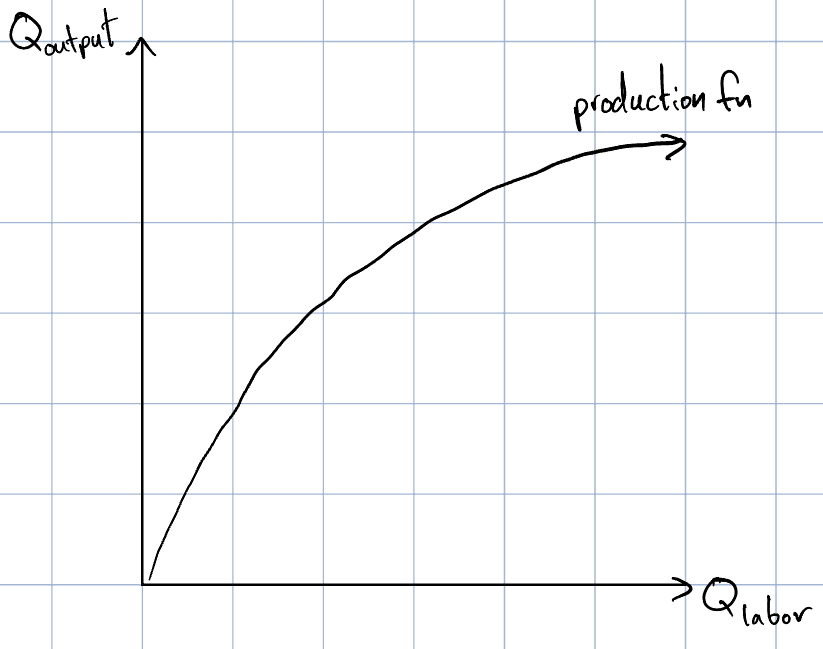
\includegraphics[width = 0.5\textwidth]{qfr4_production}
	\end{center}
	
	The total cost curve is increasing at an increasing rate because each additional unit of output requires hiring more additional labor than the last unit. That makes each additional unit of output more expensive to produce than the last.
	
	\begin{center}
	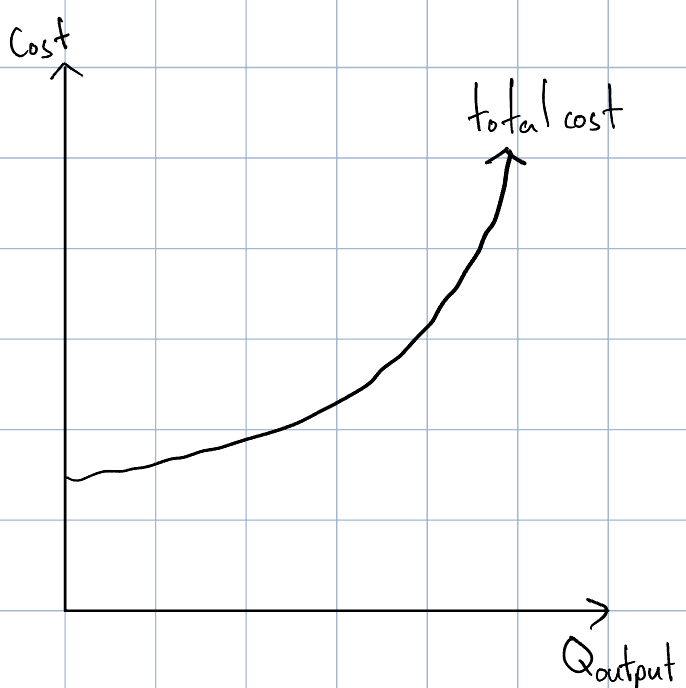
\includegraphics[width = 0.5\textwidth]{qfr4_totalcost} 
	\end{center}
	
\item Total cost is the sum of all the explicit and implicit fixed and variable costs that it takes to produce a firm's total output. Average total cost is the cost of producing a typical unit of output. Mathematically, it's total cost divided by total output. Marginal cost is the cost of producing an additional unit of output. Mathematically, it's the change in total cost divided by the change in total output.

\item \phantom{x}

	\begin{center}
	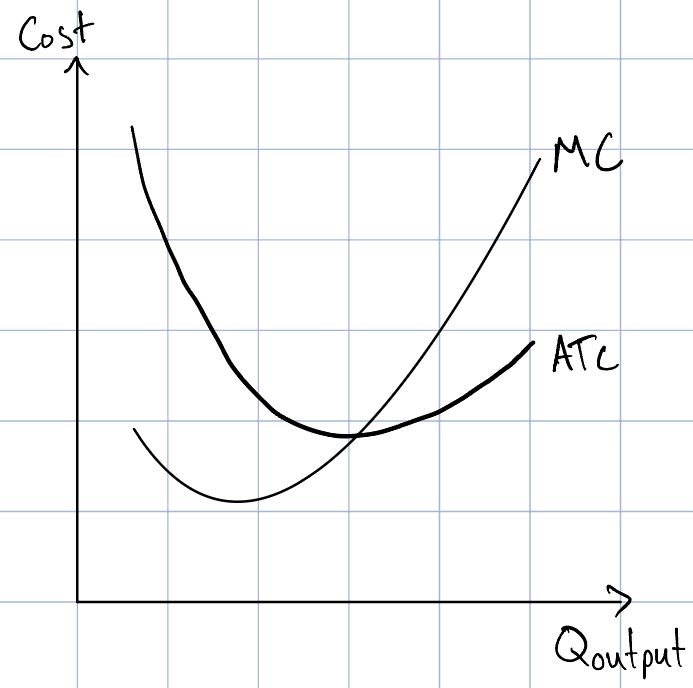
\includegraphics[width = 0.5\textwidth]{qfr6}
	\end{center}

As output increases, marginal cost typically decreases at first before eventually increasing. At first, the marginal product of labor increases because having more workers allows the workers to specialize and get better at their job. That makes marginal cost go down. Eventually, once the workers have already specialized, there's not enough equipment for additional workers to operate at maximum capacity, so the marginal product of labor diminishes which drives up marginal costs.

Average total cost has a similar U-shape. It decreases at first because average fixed cost falls quickly as the fixed costs are spread across the first few units of output. It eventually increases because diminishing marginal product causes variable costs to increase, and eventually the increase in variable costs overwhelms the decrease in fixed costs. 

The marginal cost curve intersects the average total cost curve at its minimum. If marginal cost is below average total cost, then producing an additional unit of output will pull the average total cost curve down. If marginal cost is above average total cost, then producing an additional unit of output will pull the average total cost curve up. That means the average total cost curve flips from decreasing to increasing when the marginal cost curve moves from below it to above it.

 

\end{enumerate}

\subsection*{Problems \& Applications}

\begin{enumerate}

\item

	\begin{enumerate}
	
	\item opportunity cost
	
	\item average total cost
	
	\item fixed cost
	
	\item variable cost
	
	\item total cost
	
	\item marginal cost
	
	\end{enumerate}
	
\item 

	\begin{enumerate}
	
	\item The opportunity cost of a choice is what you give up to make it.
	
	\item $\$350,000 + \$80,000 = \$430,000$
	
	\item $\$400,000 - \$350,000 = \$50,000$
	
	\item She should not. Her economic profit is negative because her opportunity cost is greater than her total revenue. In other words, she would make more money if she remained a vampire hunter. 
	
	\item It would need to generate more than her opportunity cost, \$430,000. 
	
	\end{enumerate}
	
\item

	\begin{enumerate}
	
	\item \phantom{x}
	
		\begin{center}
		\begin{tabular}{ c | c | c}
		\textbf{Hours} & \makecell{\textbf{Quantity of Fish}\\\textbf{(in pounds)}} & \makecell{\textbf{Marginal}\\ \textbf{Product}} \\
		\hline
		0 & 0 & -- \\
		1 & 10 & 10 \\
		2 & 18 & 8 \\
		3 & 24 & 6 \\
		4 & 28 & 4 \\
		5 & 30 & 2 \\
		\end{tabular}
		\end{center}
		
	\item The production function is increasing at a decreasing rate because the fisherman's marginal product of time is diminishing. The more hours he works, the less productive each additional hour is. Maybe the poor guy gets tired.
	
		\begin{center}
		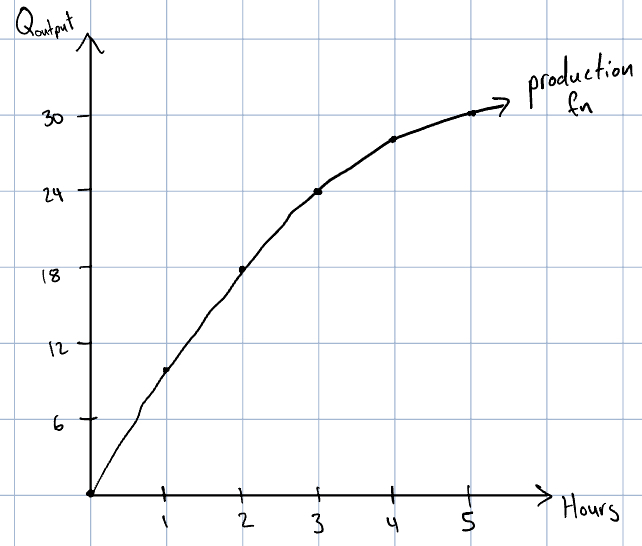
\includegraphics[width = 0.5\textwidth]{paa3b}
		\end{center}
		
	\item The total cost curve is increasing at an increasing rate. Because the fisherman's marginal product of time is diminishing, each additional fish that he catches takes him more time to catch than the last one. Since his time is worth money, that means it costs him more money to catch each additional fish.
	
		\begin{center}
		\begin{tabular}{ c | c | c | c | c }
		\textbf{Hours} & \makecell{\textbf{Quantity of Fish}\\\textbf{(in pounds)}} & \makecell{\textbf{Fixed}\\\textbf{{Cost}}} & \makecell{\textbf{Variable}\\\textbf{Cost}} & \makecell{\textbf{Total}\\\textbf{Cost}} \\
		\hline
		0 & 0 & 10 & 0 & 10 \\
		1 & 10 & 10 & 5 & 15 \\
		2 & 18 & 10 & 10 & 20  \\
		3 & 24 & 10 & 15 & 25 \\
		4 & 28 & 10 & 20 & 30 \\
		5 & 30 & 10 & 25 & 35 \\
		\end{tabular}
		
		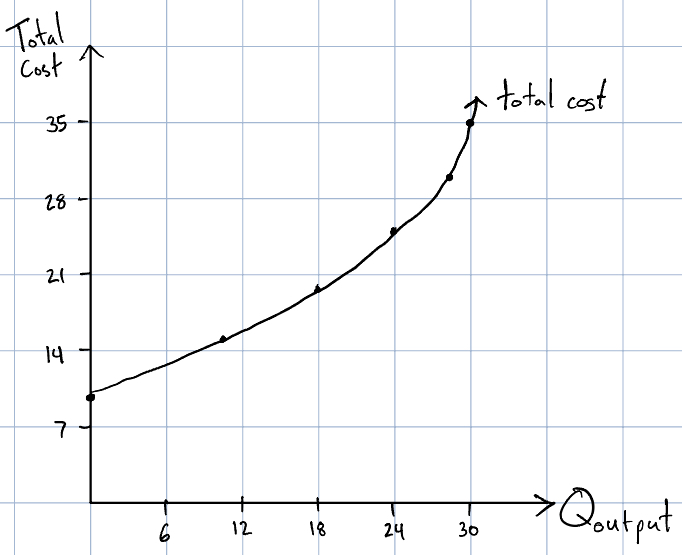
\includegraphics[width = 0.5\textwidth]{paa3c}
		\end{center}
	
	\end{enumerate}
	
\item \phantom{x}

	\begin{center}
	\begin{tabular}{| c | c | c | c | c | c |}
	\hline
	Workers & Output & \makecell{Marginal\\Product} & \makecell{Total\\Cost} & \makecell{Average\\Total\\Cost} & \makecell{Marginal\\Cost} \\
	\hline
	0 & 0 & -- & 200 & -- & -- \\
	\hline
	1 & 20 & 20 & 300 & 15 & 5 \\
	\hline
	2 & 50 & 30 & 400 & 8 & 3.33 \\
	\hline
	3 & 90 & 40 & 500 & 5.56 & 2.5 \\
	\hline
	4 & 120 & 30 & 600 & 5 & 3.33 \\
	\hline
	5 & 140 & 20 & 700 & 5 & 5 \\
	\hline
	6 & 150 & 10 & 800 & 5.33 & 10 \\
	\hline
	7 & 155 & 5 & 900 & 5.81 & 20 \\
	\hline
	\end{tabular}
	\end{center}
	
	\begin{enumerate}
	
	\item At first, marginal product is increasing. Then, it diminishes. Additional workers might be increasingly productive at first because having multiple workers allows each worker to specialize and become better at their particular task. Eventually, additional workers might become decreasingly productive because there isn't enough equipment in the factory for each worker to operate at maximum capacity. 
	
	\item See above.
	
	\item Average total cost decreases at first and increases later.
	
	\item Marginal cost decreases at first and increases later.
	
	\item Marginal product increases at first and decreases later. Marginal cost decreases at first and increases later. The trend in marginal product explains the trend in marginal cost. Since workers get increasingly productive at first, it requires less additional labor to produce an additional unit of output. Less additional labor means lower marginal costs. When workers get less productive, it requires more additional labor to produce an additional unit of output. Hiring more additional labor means higher marginal costs.
	
	\item When marginal cost is lower than average total cost, average total cost is decreasing because producing additional units at lower cost pulls the average down. When marginal cost is higher than average total cost, average total cost is increasing because producing additional units at higher cost pulls the average up.
	
	\end{enumerate}
	
\item No, I shouldn't. At 600 consoles, total cost is $600 * \$300 = \$180,000$. At 601 consoles, total cost is $601 * \$301 = \$180,901$. That means the marginal cost of producing the 601st console is \$901. That's more than the \$550 I'm being offered, so I shouldn't accept the offer.

\end{enumerate}

\end{document}